
%%%%%%%%%%%%%%%%%%%%%%%%%%%%%%%%%%%%%%%%%%%%%%%%%%%%%%%%%%
\chapter{Related Work}
\label{chapter_related_work}
%%%%%%%%%%%%%%%%%%%%%%%%%%%%%%%%%%%%%%%%%%%%%%%%%%%%%%%%%%

\mynote{
\begin{packeditems}
\item More than a literature review
\item Organize related work - impose structure
\item Be clear as to how previous work being described relates to your own. This is not just a list of the related work, you must describe how it is related. How is similar? How is it different?
\item The reader should not be left wondering why you've described something!!
\item Critique the existing work - Where is it strong where is it weak? What are the unreasonable/undesirable assumptions?
\item Identify opportunities for more research (i.e., your thesis) Are there unaddressed, or more important related topics?
\item After reading this chapter, one should understand the motivation for and importance of your thesis
\item You should clearly and precisely define all of the key concepts dealt with in the rest of the thesis, and teach the reader what s/he needs to know to understand the rest of the thesis.
\end{packeditems}
}

\mynote
{
	because it's deformation-driven thesis, 
	you need to explain deformation-driven packing vs rigid packing vs data driven packing
}

\begin{figure}[t]
\centering
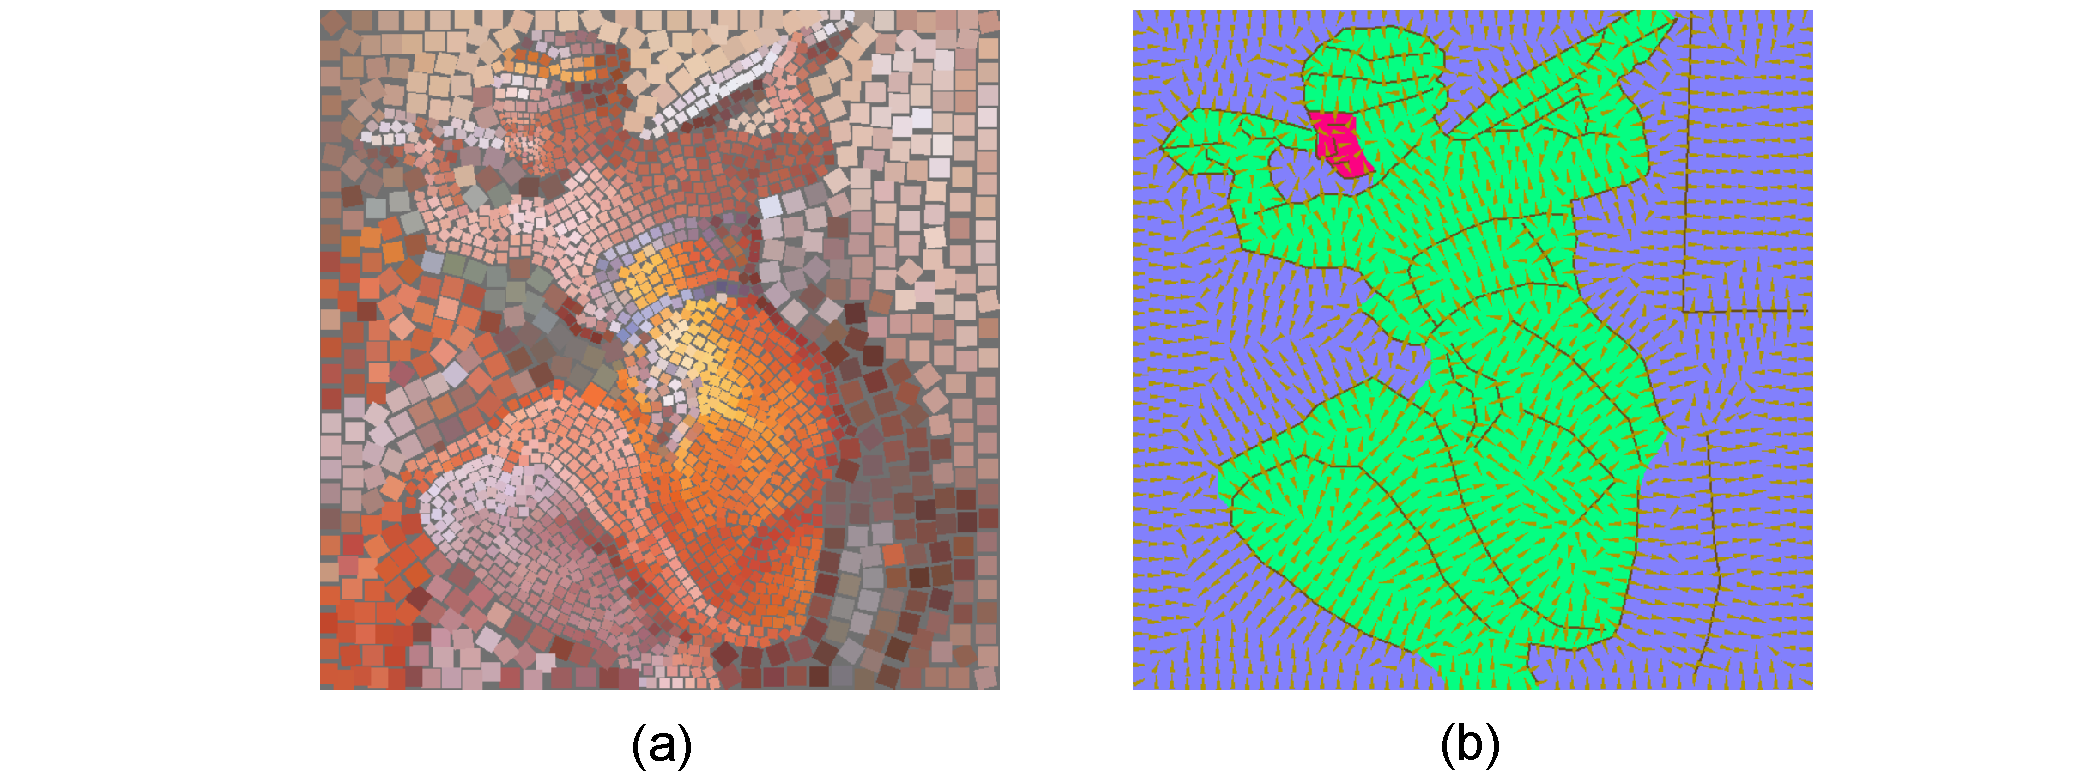
\includegraphics[width=1.0\textwidth]{figures/related/hausner.pdf} 
\caption[Decorative mosaics using Lloyd's method]
{\label{fig_related_hausner} 
Hausner. }
\end{figure}


\begin{figure}[t]
\centering
\includegraphics[width=1.0\textwidth]{figures/related/jim_pad.pdf} 
\caption[Examples of packings generated by JIM and PAD]
{\label{fig_related_jim_pad} 
JIM and PAD. }
\end{figure}

\begin{figure}[t]
\centering
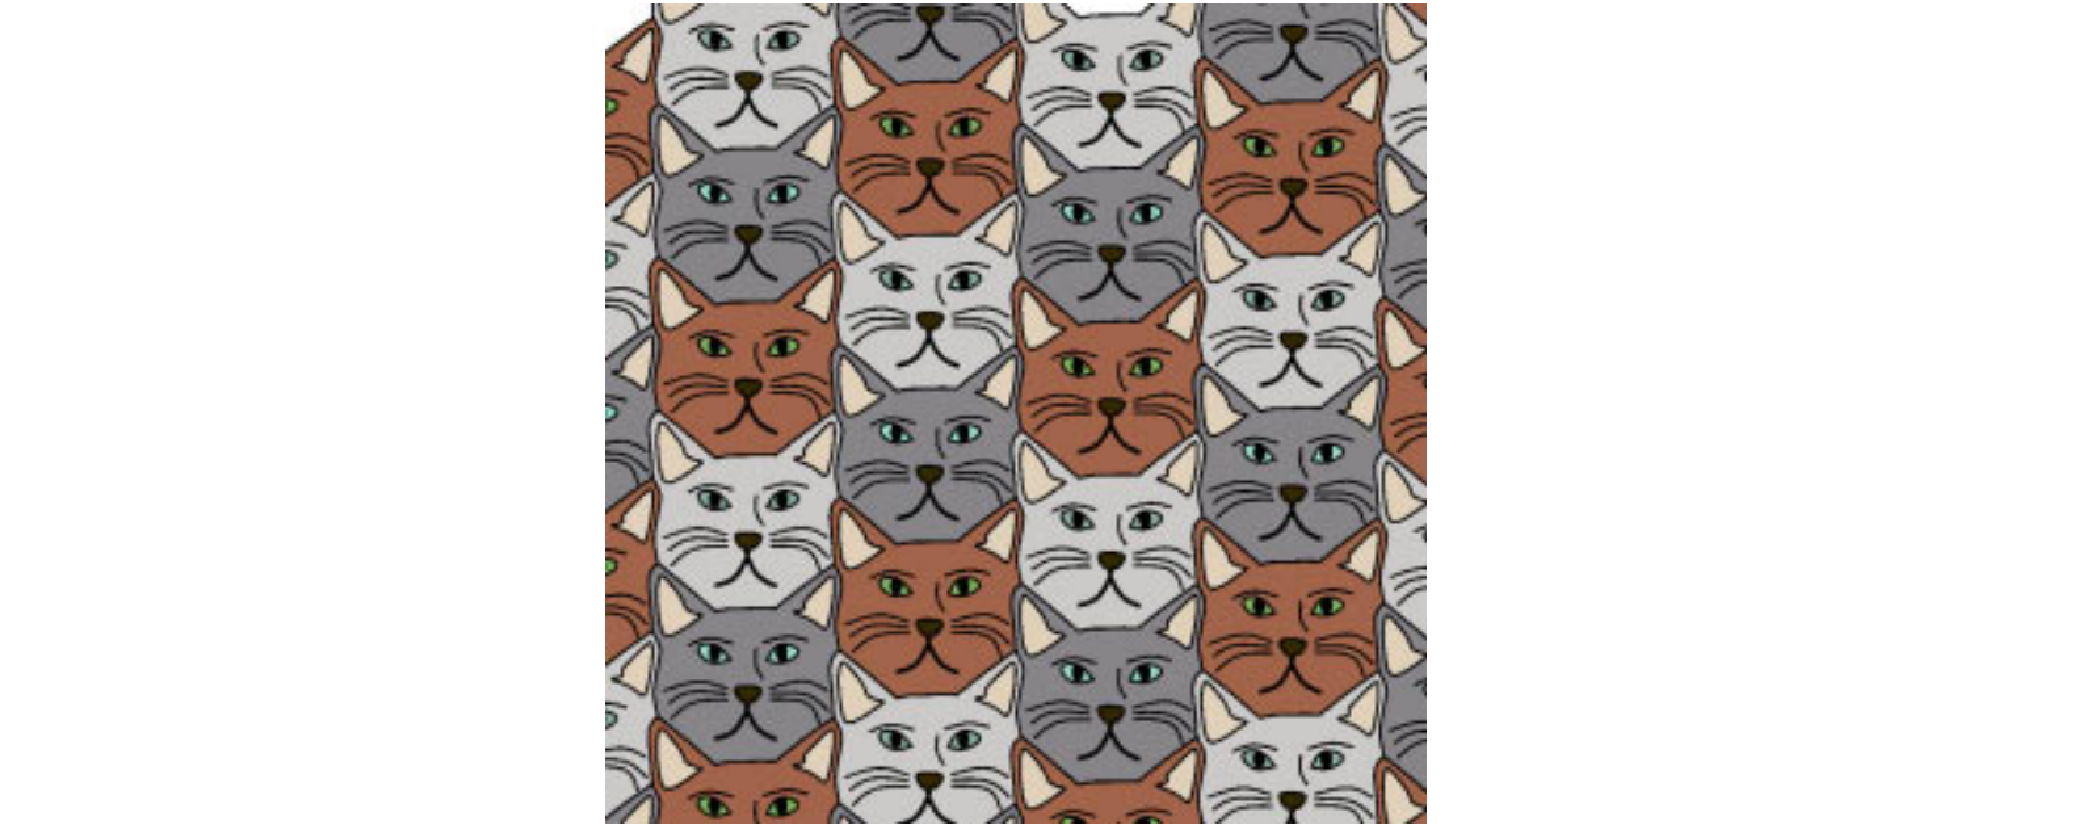
\includegraphics[width=1.0\textwidth]{figures/related/escherization.pdf} 
\caption[An example of a tiling]
{\label{fig_related_escherization} 
A tiling of cats. }
\end{figure}

\begin{figure}[t]
\centering
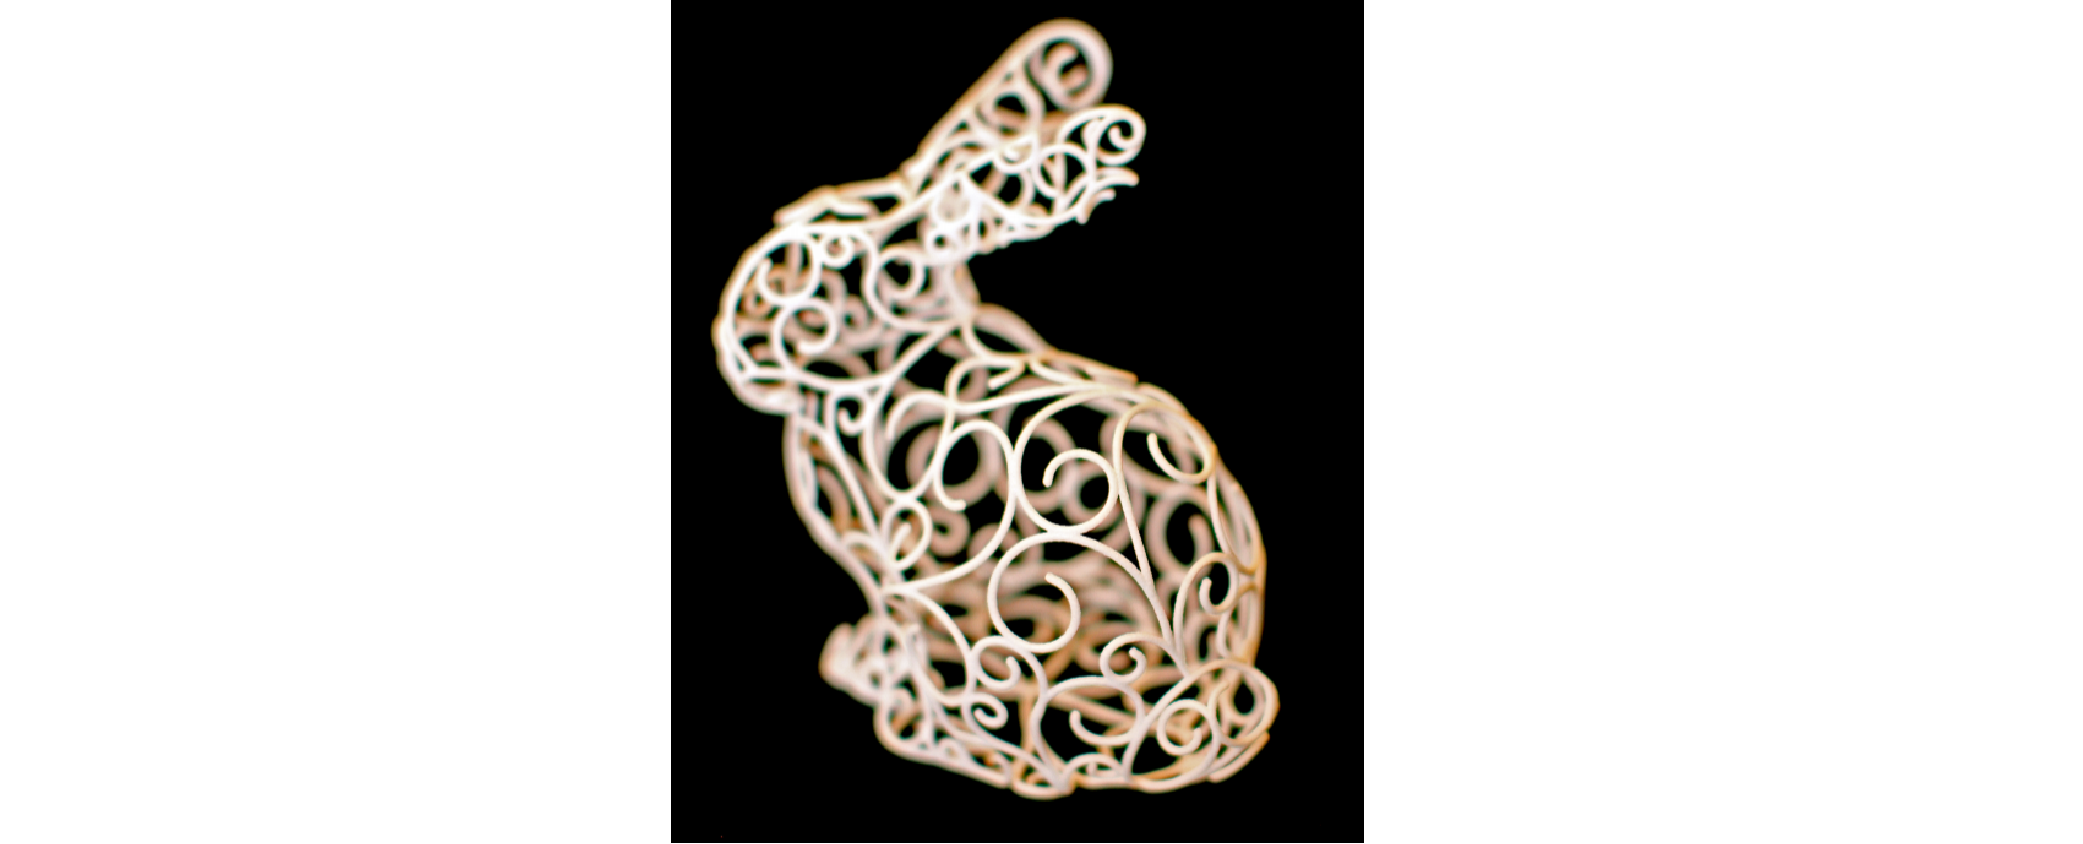
\includegraphics[width=1.0\textwidth]{figures/related/zehnder.pdf} 
\caption[An example of decorative ornaments filling a surface]
{\label{fig_related_zehnder} 
An example of decorative ornaments filling a surface.}
\end{figure}

\begin{figure}[t!]
\centering

\includegraphics[width=1.0\textwidth]{figures/related/calligraphy.pdf} 
\caption[A calligraphy packing of an ``elephant'']
{\label{fig_calligraphy} 
A calligraphy packing of an ``elephant'.}
\end{figure}


%%%%%%%%%%%%%%%%%%%%%%%%%%%%%%%%%%%%%%%%%%%%%%%%%%%%%%%%%%
\section{2D Mosaics and Packings}
%%%%%%%%%%%%%%%%%%%%%%%%%%%%%%%%%%%%%%%%%%%%%%%%%%%%%%%%%%

Rigid packing algorithms attempt to distribute elements through rigid transformations.
These algorithms can be categorized into two groups: iterative methods and data-driven methods.
Iterative methods start with an initial configuration then they use a variant of Lloyd's method 
to refine the configuration to an even distribution of elements.
data-driven methods rely on a shape matching algorithm to find a matching element from
an element library.
Some of rigid packing algorithms have an additional step where they 
correct gaps and overlaps using deformation, the deformation was applied
locally near edges in a post-processing step after elements
were frozen in place.

\textbf{Rigid packings using Lloyd's method:}
An approach to generate packing is to start with an initial configuration and iteratively refine it using Lloyd's method
to obtain an even distribution of elements. 
We first discuss the simplest example where elements are simply 2D points.
Given an initial distribution of $N$ points, 
we first compute a \textit{Voronoi diagram} to partition the plane into $N$ regions such that
all points inside a Voronoi cell are closest to its associated element.
As an iterative process, 
the Lloyd's method moves every site to the centroid of its Voronoi cell, 
then the Voronoi diagram is recomputed.
The process is repeated until the site distribution is even.
The final structure is called a \textit{Centroidal Voronoi Diagram} (CVD), 
where all the sites are located at the the centroids of the Voronoi cells.  
Originally, Lloyd's method can only distribute points.
Hausner~\cite{Hausner2001} modified the Lloyd's method to distribute square elements into a container 
region, simulating the appearance of traditional mosaics. 
This can be achieved by replacing Euclidean distance with Manhattan distance so that Voronoi cells resemble squares instead of hexagons.
However, Hausner's approach can only move these squares, but not rotate them,
so more complicated shapes such as long-shaped rectangles would have severe overlaps.
Hiller et al.~\cite{Hiller2003} extended Hausner's idea to generate \textit{Centroidal Area Voronoi Diagram} (CAVD),
a variant of CVD that accepts simple polygonal elements as input sites.
This new extension computes the principal axis for each Voronoi cell so that 
each element can be rotated to get better alignment
with its Voronoi cell boundary.
In a follow up work, Smith et al.~\cite{Smith2005} generated temporally coherent animated mosaics by utilizing CAVD.
Dalal et al.~\cite{Dalal2006} impoved upon CAVD using an FFT-based image correlation to reposition
elements iteratively, which could be seen as making more effective use of negative
space, and permitting non-convex elements to interlock more than they did in
earlier methods.


\textbf{Data driven methods:}
A different approach to generate packings is to
place elements one by one. This requires a library containing
a large number of elements. For each step, a shape matching algorithm
picks an element that has the best fit with the container boundary.
Once the element is placed, the container boundary is recomputed and
the process is repeated until the container is full.
Jigsaw Image Mosaics~\cite{Kim2002} used a geometric hashing to find
a matching element. JIM places elements using a greedy approach, but is able to backtrack 
if previous configuration is more optimal.
Pyramid of Arclength Descriptor~\cite{Kwan2016} developed
a partial shape matching algorithm that can match a subset of element boundary with a portion
of container boundary.
%Gal et al.~\cite{Gal2007B} presented a method for constructing 3D
%collages reminiscent of portrait paintings by Arcimboldo.  They
%filled a 3D container with overlapping 3D elements using a greedy
%approach and a partial shape matching algorithm. 

It is also possible to partition the container into smaller segments,
then use a shape matching algorithm to replace each segment with
a matching element.
Huang et al.~\cite{Huang2011} produced Arcimboldo-like collages
by arranging cutout images taken from the internet.
Their container is a bigger cutout image which is partitioned into segments
using an image segmentation algorithm.
Each segment is then replaced with a cutout image that has a similar shape and color.

All three methods above the element library to big enough,
the more elements in the library will increase their chance to find a compatible element boundary.
However, bigger database means increased computational time.
Collecting a large number of elements is also not always feasible,
for example, if an artist wants to create a packing of a hand-drawn cats,
they may not want to draw 1000 cats which is tedious and repetitive.

%%%%%%%%%%%%%%%%%%%%%%%%%%%%%%%%%%%%%%%%%%%%%%%%%%%%%%%%%%
\section{Non-rigid Packing Methods}
%%%%%%%%%%%%%%%%%%%%%%%%%%%%%%%%%%%%%%%%%%%%%%%%%%%%%%%%%%


Peng et al.~\cite{Peng2014} computed layouts by packing and deforming
simple polygons and polyominoes. Their method cannot handle more
complicated shapes, making it unsuitable for our style of packings.
Xu and Kaplan~\cite{Xu2007} and Zou et al.~\cite{Zou2016}
constructed \textit{calligrams} by filling a container with a small
number of deformed letters composing one or two words.  Because the
order of the letterforms was defined by the text, their solutions
usually required significant distortion of the individual letters.
Their goal was to balance between filling the container and preserving
readability.
Zehnder et al.~\cite{Zehnder2016} proposed an method to
cover 3D surfaces with deformed ornamental elastic curves.



%%%%%%%%%%%%%%%%%%%%%%%%%%%%%%%%%%%%%%%%%%%%%%%%%%%%%%%%%%
\section{Tilings}
%%%%%%%%%%%%%%%%%%%%%%%%%%%%%%%%%%%%%%%%%%%%%%%%%%%%%%%%%%
\mynote{dihedral escherization}
Kaplan and Salesin~\cite{Kaplan2000} deformed a single user-supplied 
input shape into one that could tile the plane.

%%%%%%%%%%%%%%%%%%%%%%%%%%%%%%%%%%%%%%%%%%%%%%%%%%%%%%%%%%
\section{3D Packings}
%%%%%%%%%%%%%%%%%%%%%%%%%%%%%%%%%%%%%%%%%%%%%%%%%%%%%%%%%%
% moved to data driven
%Gal et al.~\cite{Gal2007B} presented a method for constructing 3D
%collages reminiscent of portrait paintings by Arcimboldo.  They
%filled a 3D container with overlapping 3D elements using a greedy
%approach and a partial shape matching algorithm.

% this one is too narrow, kinda unrelated
%Attene~\cite{Attene2015} decomposed a 3D model into parts that pack
%tightly into a small build volume, allowing it to 
%be 3D printed with less waste material and packed into a smaller box.

Ma et al.~\cite{Ma2018} developed a heuristic method
to create 3D packings that are overlap free.

%%%%%%%%%%%%%%%%%%%%%%%%%%%%%%%%%%%%%%%%%%%%%%%%%%%%%%%%%%
\section{Discrete Texture Synthesis}
%%%%%%%%%%%%%%%%%%%%%%%%%%%%%%%%%%%%%%%%%%%%%%%%%%%%%%%%%%
Some past work has sought to adapt example-based texture synthesis methods
from raster images to vector graphics, producing distributions of rigidly transformed elements
that mimic the statistics of an exemplar.  Barla et al.~\cite{Barla2006} and
Ijiri et al.~\cite{Ijiri2008} use a growth model that copies small neighbourhoods
from the exemplar into a larger output texture.  AlMeraj et al.~\cite{AlMeraj2013}
stamp out copies of the exemplar and discard overlapping elements.
Hurtut et al.~\cite{Hurtut2009} develop a statistical sampling method based
on multitype point processes.  
These techniques are all concerned with replicating
the uneven element distribution in the exemplar, without regard for negative space.

%%%%%%%%%%%%%%%%%%%%%%%%%%%%%%%%%%%%%%%%%%%%%%%%%%%%%%%%%%
\section{Packings on Surfaces}
%%%%%%%%%%%%%%%%%%%%%%%%%%%%%%%%%%%%%%%%%%%%%%%%%%%%%%%%%%
Related work in fabrication has sought to cover surfaces with
arrangements of deformed ornamental elements that satisfy manufacturing
constraints such as connectivity.  Chen et al.~\cite{Chen2016}
developed a method to synthesize filigree patterns out of simple
elements. 
In later work, Chen et al.~\cite{Chen2017}
generated modular surfaces by computing 
contact point networks of rigid elements.
\mynote{zehnder}
\mynote{Surface Mosaic Synthesis with Irregular Tiles}




